\renewcommand{\LifeChapter}{y}
\chapter{Introduction}
\label{chap:introduction}

\chaptertoc{}

\begin{chapterabstract}
  This purpose of this chapter abstract is to describe what the chapter is about.
\end{chapterabstract}

\section{Motivation}
\label{sec:intro_motivation}
\Blindtext

\begin{figure}
  \centering
  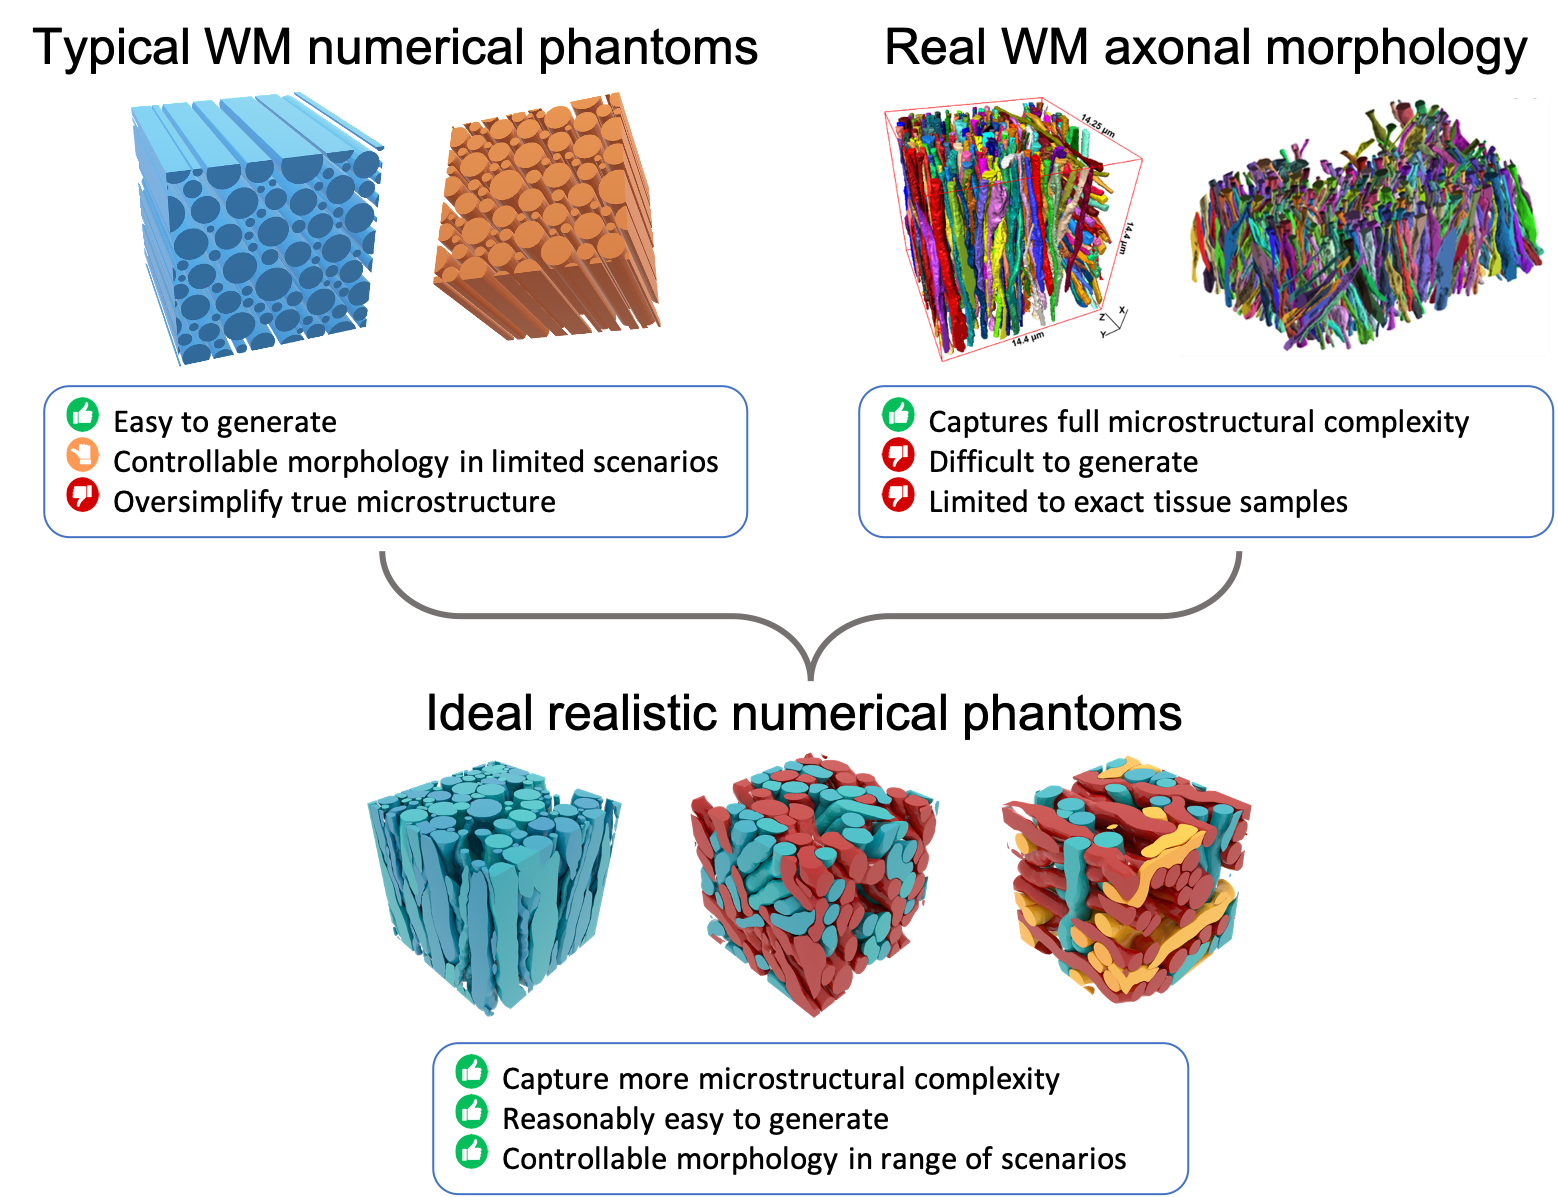
\includegraphics[width=\textwidth]{figures/introduction/overview}
  \caption[Overview of the main goal of the thesis]{This is a figure caption}
  \label{fig:intro_overview}
\end{figure}

\section{Problem Statement}
\label{sec:intro_problem_statement}
\blindtext


\section{Project Aims and Scope}
\label{sec:intro_project_aims}
\blindtext

 

The mains aims of this work are as follows:
\blindenumerate




\section{Report Overview}
\label{sec:intro_report_overview}
The rest of the report is arranged as follows: \Cref{chap:background} shows some text with math and \Cref{chap:conclusion} shows a chapter in a new part of the thesis.



%%% Local Variables:
%%% mode: latex
%%% TeX-master: "../main"
%%% End:
